\documentclass[11pt,a4paper]{article}
\usepackage[T1]{fontenc}
\usepackage[utf8]{inputenc}
\usepackage{lmodern}
\usepackage[margin=25mm]{geometry}
\usepackage{amsmath,amssymb,amsthm,mathtools}
\usepackage{microtype,graphicx,booktabs}
\usepackage[numbers,sort&compress]{natbib}
\usepackage[colorlinks=true,linkcolor=blue,citecolor=blue,urlcolor=blue]{hyperref}
\hypersetup{pdftitle={Finite total dephasing and an isolated natural occupation in an open XX chain},pdfauthor={Xiaojian Zeng}}
\newcommand{\D}{\mathcal{D}}
\newcommand{\sgn}{\operatorname{sgn}}
\newcommand{\IPR}{\operatorname{IPR}}
\newcommand{\tr}{\operatorname{Tr}}
\newcommand{\ii}{\mathrm{i}}
\newcommand{\Id}{\mathbb{I}}
\newtheorem{proposition}{Proposition}
\title{Finite total dephasing and an isolated natural occupation in an open XX chain}
\author{Xiaojian Zeng\\[3pt]
\small PBC School of Finance, Tsinghua University, 100190\\
\small \href{mailto:xiaojianzeng@foxmail.com}{xiaojianzeng@foxmail.com}}
\date{}

\begin{document}
\maketitle
\begin{abstract}
We study the stationary one-particle covariance of an open XX spin chain
with unequal end reservoirs, a central dephasing defect, and weak
dephasing distributed over the chain. The background is scaled so that
its total phase-flip event rate stays finite as the chain grows. For
fixed specified boundary and defect strengths, an exactly half-occupied
natural orbital remains separated from all other natural occupations.
We obtain its limiting occupation spacing as an explicit positive
function of the total noise strength, while its inverse participation
ratio approaches a noise-independent value. Center-deletion interlacing
and a two-dimensional sine trial space control the occupation spacing;
an orbital residual estimate controls convergence of the normalized
mode. The estimates address a spatially nonuniform limit in which the
local background vanishes but the integrated resistance changes by a
finite amount. The known zero-background exponential profile survives
this limit. All limits are taken after stationarity at each finite size,
and concern covariance occupations rather than relaxation rates.
\end{abstract}
\noindent\textit{Keywords:} Quantum Dissipative Systems;
Spin chains, ladders and planes

\section{Introduction}
Boundary-driven XX chains provide explicit examples of nonequilibrium
transport modified by dephasing. The uniform-dephasing stationary
magnetization and current are known exactly at arbitrary reservoir
bias~\cite{Znidaric2010}. Related harmonic chains admit a tridiagonal
stationary covariance and an additive dephasing resistance~\cite{Asadian2013}.
These moment structures make spectral questions about the covariance
accessible, even when the full stationary density operator is more
complicated.

The eigenvalues of an equal-time one-particle covariance are natural
occupations. They differ from the spectrum of the generator that evolves
the correlator, as studied, for example, by Alba~\cite{Alba2025}.
Closed two-point dynamics also do not imply a Gaussian many-body state;
local dephasing can generate non-Gaussian correlations~\cite{Dolgirev2020}.
Thus spectral isolation of one natural occupation has a precise
one-particle meaning, without implying a many-body relaxation gap or an
entanglement property.

Here the background noise has a finite total event rate, distributed
uniformly over an increasing number of sites. The noise at each fixed
site then vanishes, whereas its contribution to the stationary
resistance remains finite. This distinction raises a question that a
current formula alone does not settle: can a localized natural orbital
retain both its shape and a nonzero separation from the other
occupations? We answer it on one specified parameter slice, with a
central defect in odd open chains. The zero-background geometric profile
is already related by site phases to the familiar imaginary-impurity
mode~\cite{Kokkinakis2026}. The contribution here is its joint orbital and
occupation-spacing limit under finite distributed noise, together with
finite-size bounds. Neither the resistance law nor the exponential
profile is a new ingredient.

\section{Spin model and the finite noise rate}
Consider $N=2L+1\ge3$ spin-$1/2$ sites on an open path. In units with
$\hbar=1$, the Hamiltonian and canonical dissipator are
\begin{align}
 H&=J\sum_{j=1}^{N-1}
 (\sigma_j^x\sigma_{j+1}^x+\sigma_j^y\sigma_{j+1}^y),\qquad J>0,
 \label{eq:H}\\
 \frac{d\rho}{ds}&=-\ii[H,\rho]+\sum_a\D[L_a]\rho,
 &\D[A]\rho&=A\rho A^\dagger-\tfrac12\{A^\dagger A,\rho\}.
 \label{eq:GKSL}
\end{align}
Here $s$ is physical time. With
$\sigma^\pm=(\sigma^x\pm\ii\sigma^y)/2$, the end jumps are
\begin{equation}
 L_b^+=\sqrt{\kappa f_b}\,\sigma_b^+,
 \qquad L_b^-=\sqrt{\kappa(1-f_b)}\,\sigma_b^-,
 \qquad b=1,N,
 \label{eq:baths}
\end{equation}
where $f_1=(1-\mu)/2$ and $f_N=(1+\mu)/2$. These are target local
occupations of Markovian spin reservoirs. The dephasing jumps are
\begin{equation}
 L_j^z=\sqrt{\gamma_j/2}\,\sigma_j^z,
 \qquad \gamma_j=\gamma_0+\eta\delta_{j,L+1}.
 \label{eq:dephasing}
\end{equation}
All rates and $J$ have units of inverse time; jump amplitudes have units
of inverse square-root time. We fix throughout
\begin{equation}
 \kappa=4J,\qquad \mu=\tfrac12,\qquad \eta=5J,
 \qquad \gamma_0=Jq_N,
 \label{eq:parameters}
\end{equation}
and consider, for each fixed finite dimensionless $c>0$, either
\begin{equation}
 q_N=\frac{c}{N}\quad\hbox{or}\quad q_N=\frac{c}{N-1}.
 \label{eq:scalings}
\end{equation}
Equivalently, one may measure time in $J^{-1}$ and write $J=1$,
$\kappa=4$, $\eta=5$. In a convention using a dimensional noise
parameter $c_{\rm phys}$, the $c$ in this article is $c_{\rm phys}/J$.

The first scaling has a direct stochastic realization. A Poisson clock
of rate $Jc/2$ chooses one of the $N$ sites uniformly and applies its
Pauli $Z$ operator. Averaging these events produces
\begin{equation}
 \mathcal L_{\rm bg}\rho=
 \frac{Jc}{2N}\sum_{j=1}^N(\sigma_j^z\rho\sigma_j^z-\rho),
 \label{eq:clock}
\end{equation}
which is exactly the background in Eq.~\eqref{eq:dephasing}.
The defect contributes a separate local clock of rate $5J/2$.
For $q_N=c/(N-1)$ the background event rate is
$JcN/[2(N-1)]$, while the bond-weighted background damping
$2(N-1)\gamma_0$ is exactly $2Jc$. Both event rates tend to $Jc/2$.
This realization is defined separately for every finite chain; it does
not require a uniform choice from an infinite set of sites.

Define Jordan--Wigner operators and the covariance by
\begin{equation}
 c_j=\left[\prod_{k<j}(-\sigma_k^z)\right]\sigma_j^- ,
 \qquad G_{jk}(s)=\tr(\rho(s)c_k^\dagger c_j).
 \label{eq:G}
\end{equation}
In particular $G_{jj}=(1+\langle\sigma_j^z\rangle)/2$.
We first take $s\to\infty$ at fixed $N$ and denote the limit by $G_N$.
Its eigenvalues $\nu_a$ lie in $[0,1]$. The size limit below is always
taken after this stationary limit.

\section{Exact stationary reduction}
The spin adjoint generator closes on the bilinears in Eq.~\eqref{eq:G}:
\begin{equation}
 \dot G_{jk}=
 \left[-\ii(hG-Gh)-\tfrac12\{K,G\}+P\right]_{jk}
 -(\gamma_j+\gamma_k)(1-\delta_{jk})G_{jk},
 \label{eq:moment}
\end{equation}
where $h_{j,j+1}=h_{j+1,j}=2J$,
$K=\operatorname{diag}(\kappa,0,\ldots,0,\kappa)$, and
$P=\operatorname{diag}(\kappa f_1,0,\ldots,0,\kappa f_N)$.
Conjugating a bilinear by $\sigma_\ell^z$ changes its sign precisely
when $j\ne k$ and $\ell$ is one of its two endpoints. This yields the
last term, which damps off-diagonal entries and leaves densities
unchanged directly. The end-spin dissipators give the displayed $K$
and $P$ terms; the Jordan--Wigner string is retained in making this
spin calculation. There is no replacement of the right spin bath by
an assumed full-state fermion bath.

For completeness, write $v=2J$, $k_j=K_{jj}$, and
\begin{equation}
 d_j=\gamma_j+\gamma_{j+1}+\tfrac12(k_j+k_{j+1}),\qquad
 \mathcal R=\frac{4v^2}{\kappa}+\sum_{j=1}^{N-1}d_j,
 \qquad a=\frac{\mu v}{\mathcal R}.
 \label{eq:resistance}
\end{equation}
The stationary solution has only a diagonal and adjacent coherences:
\begin{align}
 (G_N)_{j,j+1}&=-\ii a,&
 (G_N)_{jj}&=f_1+\frac{2va}{\kappa}
                  +\frac{a}{v}\sum_{\ell<j}d_\ell,
 \label{eq:stationary}\\
 (G_N)_{jk}&=0&&\text{for }|j-k|>1.
 \nonumber
\end{align}
The first off-diagonal equation reduces to
$v[(G_N)_{j+1,j+1}-(G_N)_{jj}]=a d_j$.
The diagonal equations express constant bond current, the second
off-diagonal terms cancel because $a$ is constant, and the right
boundary equation fixes $\mathcal R$ as in Eq.~\eqref{eq:resistance}.
This is the familiar tridiagonal moment construction and additive
resistance structure~\cite{Znidaric2010,Asadian2013}.
No expansion in $\mu$, $\eta$, or $\gamma_0$ is used here.

The covariance does converge at each finite $N$. Let $\mathcal T$ be
the homogeneous part of Eq.~\eqref{eq:moment}. Its Hilbert--Schmidt
dissipation form is
\begin{equation}
 \operatorname{Re}\langle X,\mathcal T X\rangle
 =-\tfrac12\sum_{jk}(k_j+k_k)|X_{jk}|^2
  -\sum_{j\ne k}(\gamma_j+\gamma_k)|X_{jk}|^2\le0.
 \label{eq:decay}
\end{equation}
If an eigenmatrix had an eigenvalue with zero real part, its boundary
rows and columns would vanish. Its first-row equation would then force
the second row to vanish because $v>0$. Repeating this argument along
the open path forces the entire matrix to vanish. Every eigenvalue of
$\mathcal T$ therefore has negative real part, which proves the
finite-dimensional covariance convergence. Positivity of the finite
spin evolution and the canonical anticommutation relations give
$0\le G_N\le\Id$. This argument makes no claim about a size-independent
decay rate of the many-body state.

Gauge the covariance by $U_{jj}=\ii^{j-1}$ and index sites by
$m=j-L-1$. Under Eq.~\eqref{eq:parameters}, Eqs.~\eqref{eq:resistance}
and \eqref{eq:stationary} become
\begin{equation}
 G_N'=U^\dagger G_NU=\tfrac12\Id+\frac{B_N}{R_N},
 \qquad R_N=\frac{\mathcal R}{J}=18+2(N-1)q_N,
 \label{eq:reduction}
\end{equation}
where $B_N$ is a real symmetric tridiagonal matrix with
\begin{equation}
 (B_N)_{m,m+1}=1,\qquad
 (B_N)_{mm}=q_Nm+\tfrac52\sgn(m)+\sgn(m)\delta_{|m|,L}.
 \label{eq:B}
\end{equation}
Both $B_N$ and $R_N$ are dimensionless. The linear diagonal term is a
representation of the stationary density gradient. No magnetic field
has been added to the Hamiltonian.

\section{Occupation spacing and its finite-size bound}
Let $\lambda_+(N)$ be the smallest positive eigenvalue of $B_N$.
Reflection combined with alternating site signs anticommutes with
$B_N$. An irreducible real Jacobi matrix has simple eigenvalues: its
first component fixes an eigenvector by recurrence and cannot vanish.
The odd-dimensional spectrum consequently consists of $L$ pairs of
opposite eigenvalues and one simple zero. Thus $G_N$ has a unique
occupation at $1/2$. Define
\begin{equation}
 \delta\nu_N=\min_{\nu_a\ne1/2}|\nu_a-\tfrac12|
            =\frac{\lambda_+(N)}{R_N}.
 \label{eq:gapdef}
\end{equation}

\begin{proposition}
For the model and parameters in Eqs.~\eqref{eq:H}--\eqref{eq:scalings},
each fixed finite $c>0$ has
\begin{equation}
 \lim_{\substack{N\to\infty\\N\ \mathrm{odd}}}\delta\nu_N
       =\frac{1}{36+4c}.
 \label{eq:gaplimit}
\end{equation}
For every integer $2\le M<L$, the finite-chain enclosure is
\begin{equation}
 \tfrac12+q_N\ \le\ \lambda_+(N)\ \le\
 \tfrac52+q_NM-2\cos\!\left(\frac{2\pi}{M+1}\right).
 \label{eq:gapbound}
\end{equation}
The lower bound also holds when no such $M$ exists.
\end{proposition}

\begin{proof}
Delete the central row and column of $B_N$. The right block $T$ has
diagonal $5/2+q_N j+\delta_{j,L}$, $1\le j\le L$, and unit
off-diagonal entries. The left block is unitarily equivalent to $-T$.
Write the ordered eigenvalues of $T$ as $\beta_1<\cdots<\beta_L$.
The path adjacency has operator norm at most $2$, so
$\beta_1\ge1/2+q_N>0$. Cauchy interlacing, with the exact central
zero counted, gives
\begin{equation}
 \beta_1\le\lambda_+(N)\le\beta_2\qquad(L\ge2).
 \label{eq:interlacing}
\end{equation}
For $L=1$ interlacing still gives the lower bound.

To bound $\beta_2$, take the two lowest sine eigenmodes of the
length-$M$ unit-hopping path and extend them by zero to the rest of
$T$. This two-dimensional trial space avoids the endpoint shift
because $M<L$. On its support the diagonal is at most $5/2+q_NM$;
the largest adjacency Rayleigh quotient within the space is
$-2\cos[2\pi/(M+1)]$. The second min--max principle proves the
upper bound in Eq.~\eqref{eq:gapbound}. A single trial vector would
not suffice for this second-eigenvalue estimate.

For sufficiently large $N$, choose $M=\lfloor N^{1/3}\rfloor$.
It is admissible, and
\begin{equation}
 0\le\lambda_+(N)-\tfrac12
 \le q_NM+\frac{4\pi^2}{(M+1)^2}\longrightarrow0.
 \label{eq:edgeconvergence}
\end{equation}
Since $R_N\to18+2c$, Eq.~\eqref{eq:gaplimit} follows.
\end{proof}

The upper excess is $O(N^{-2/3})$ for fixed $c$; the constants are
not asserted to be uniform in unbounded $c$. The trial-space argument
is needed because $q_Nm$ remains of order one near the remote ends,
despite vanishing at every fixed $m$.

\section{Convergence of the normalized orbital}
Let $u_N$ be the normalized zero eigenvector of $B_N$ and define
$\IPR(u)=\sum_m|u_m|^4$. The physical natural orbital is $Uu_N$,
which has the same IPR. Set $z=1/2$ and introduce a normalized
finite truncation of the zero-background profile:
\begin{align}
 w_0&=C_L,& w_{-m}&=C_Lz^m,& w_m&=C_L(-z)^m\quad(1\le m\le L),
 \label{eq:w}\\
 C_L^{-2}&=1+2\sum_{m=1}^{L}z^{2m}.
 \nonumber
\end{align}
The infinite profile solves the bulk step recurrence because
$z+z^{-1}=5/2$. Its finite-chain residual has a background part
$q_Nm w_m$ and endpoint terms of magnitude
$(1+z)C_Lz^L$. Hence
\begin{align}
 \epsilon_L:=\|B_Nw\|_2
 &\le q_N\left(\sum_m m^2|w_m|^2\right)^{1/2}
       +\sqrt2(1+z)C_Lz^L
 \label{eq:residual}\\
 &\le q_N\sqrt{8/9}+\sqrt2(1+z)C_Lz^L.
 \nonumber
\end{align}
The second moment of the infinite normalized geometric distribution
is $8/9$. Truncation conditions that distribution on $|m|\le L$,
which can only decrease its second moment.

All nonzero eigenvalues of $B_N$ have magnitude at least
$g_N=1/2+q_N$. Spectral decomposition therefore gives
\begin{equation}
 \|(\Id-u_Nu_N^\dagger)w\|_2\le\epsilon_L/g_N,
 \qquad \|u_N-w\|_2\le\sqrt2\,\epsilon_L/g_N,
 \label{eq:vectorbound}
\end{equation}
where the phase of $u_N$ is chosen to make
$\langle u_N,w\rangle\ge0$. The second inequality follows from
$2(1-\sqrt{1-r^2})\le2r^2$ for the norm $r$ of the perpendicular
component. On the unit ball, the Euclidean norm of the gradient of
$\sum_m|x_m|^4$ is at most $4$. Thus
\begin{equation}
 |\IPR(u_N)-\IPR(w)|\le
       \frac{4\sqrt2\,\epsilon_L}{1/2+q_N}.
 \label{eq:iprbound}
\end{equation}
This bound is valid even when its right-hand side is larger than one.

For either scaling in Eq.~\eqref{eq:scalings}, the right-hand side
vanishes as $O(N^{-1})$ plus an exponentially small boundary term.
The truncated vector converges in $\ell^2$, after embedding about
the center, to the normalized infinite geometric vector. Summing its
fourth powers gives the second limiting result,
\begin{equation}
 \lim_{\substack{N\to\infty\\N\ \mathrm{odd}}}\IPR(u_N)
 =\frac{(1-z^2)(1+z^4)}{(1+z^2)^3}
 =\frac{51}{125}.
 \label{eq:iprlimit}
\end{equation}
Its central probability is $3/5$ and the probabilities decrease by a
factor $1/4$ per site away from the center. In the ungauged basis the
amplitudes are proportional to $(-\ii/2)^{|m|}$, up to an overall
phase. This is the known imaginary-impurity exponential
profile~\cite{Kokkinakis2026}; identifying it here does not identify
the covariance spectrum with a non-Hermitian energy spectrum.

\section{Finite-size illustration and physical consequence}
Figure~\ref{fig:convergence} shows the approach to both limits for
$q_N=c/N$ at $c=1/2$ and $c=2$. It uses $N=81,161,321,641,1281,2561$.
The numerical eigenpairs come from a real symmetric tridiagonal
eigensolver, retaining the exact reflection pattern when assembling
the diagonal. The plotted upper occupation bound minimizes
Eq.~\eqref{eq:gapbound} over all admissible integers $M$. The IPR
bound evaluates Eq.~\eqref{eq:iprbound} and adds
$|\IPR(w)-51/125|$.

\begin{figure}[t]
 \centering
 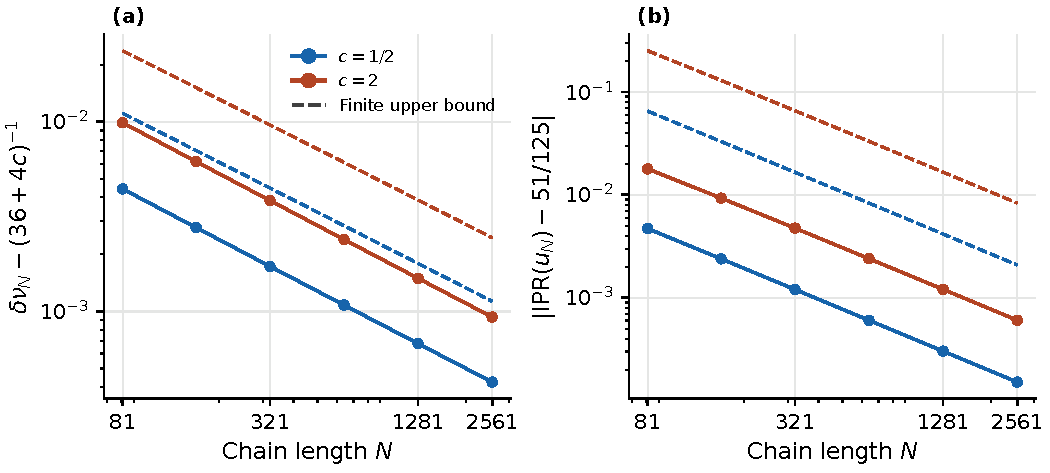
\includegraphics[width=\linewidth]{figures/convergence.pdf}
 \caption{Finite-size deviations from the stationary-first limits at
 $\kappa/J=4$, $\mu=1/2$, $\eta/J=5$, and $q_N=c/N$.
 (a) Occupation-spacing excess. (b) Absolute IPR error. Solid lines
 join numerical values, and dashed lines evaluate the finite upper
 bounds in Eqs.~\eqref{eq:gapbound} and \eqref{eq:iprbound}.
 Both axes in each panel are logarithmic. The bounds are not fitted
 to the data. Floating-point evaluations illustrate the analytic
 inequalities; they are not interval enclosures.}
 \label{fig:convergence}
\end{figure}

The calculation includes both normalizations in
Eq.~\eqref{eq:scalings}, giving 24 cases. At the four largest-size
cases, an 80-digit boundary recurrence checks the zero-orbital IPR,
and an alternate tridiagonal QR method checks the spacing. The
accompanying code records the residuals and discrepancies. These are
numerical precision checks; Eqs.~\eqref{eq:edgeconvergence} and
\eqref{eq:iprbound} establish the limits independently of the table.

\begin{table}[t]
 \centering
 \caption{Finite values at $N=2561$ for both background conventions.
 All quantities displayed are dimensionless, and numerical entries
 are rounded to nine decimal places. The limiting IPR is $0.408$ in
 every row. The difference between a finite value and its limit is
 a size effect, not an estimated numerical uncertainty.}
 \label{tab:finite}
 \begin{tabular}{ccccc}
\toprule
$c$ & $q_N$ & $\delta\nu_N$ & $(36+4c)^{-1}$ & $\IPR(u_N)$\\
\midrule
$1/2$ & $c/(N-1)$ & 0.026739105 & 0.026315789 & 0.408151461 \\
$2$ & $c/(N-1)$ & 0.023659581 & 0.022727273 & 0.408604709 \\
$1/2$ & $c/N$ & 0.026739543 & 0.026315789 & 0.408151401 \\
$2$ & $c/N$ & 0.023661015 & 0.022727273 & 0.408604473 \\
\bottomrule
\end{tabular}

\end{table}

Table~\ref{tab:finite} also shows that the occupation-spacing limit
is approached more slowly than the IPR limit. Even at $N=2561$,
the spacing differs from its limit by about $1.6\%$ for $c=1/2$
and $4.1\%$ for $c=2$. The two finite-size normalizations give
slightly different values while sharing both limits.

The joint result separates the effects of distributed noise on an
orbital and on its occupation environment. For the specified defect,
the local orbital shape converges to the zero-background shape,
but the denominator $R_N$ retains the finite background contribution
$2c$. The occupation separation is consequently reduced to
$(36+4c)^{-1}$ while the IPR remains $51/125$.

At fixed positive noise per site, the conclusion about the spacing
changes. Keeping $q_N=q>0$ and taking $M=2$ in
Eq.~\eqref{eq:gapbound} gives, for $L>2$,
\begin{equation}
 \frac{1/2+q}{18+2(N-1)q}
 \le\delta\nu_N\le
 \frac{7/2+2q}{18+2(N-1)q}.
 \label{eq:fixedq}
\end{equation}
Thus the spacing has order $N^{-1}$ in that limit. The nonzero
limit in Eq.~\eqref{eq:gaplimit} is specifically a finite-total-rate
statement, rather than stability of the occupation separation under
fixed positive dephasing at every site.

\section{Conclusion}
For an odd open XX chain with a centered defect and the fixed rates
in Eq.~\eqref{eq:parameters}, finite distributed phase-flip rate
preserves an isolated half-occupied natural orbital. Its spacing tends
to $(36+4c)^{-1}$ while its normalized IPR tends to $51/125$.
Interlacing and a two-mode variational estimate control the spectral
edge despite the nonvanishing diagonal variation far from the
center. A residual estimate separately controls the orbital norm
and IPR. These provide finite-size benchmarks for stationary
one-particle calculations in this specified noise model.

The result concerns neither a Liouvillian gap nor an excitation
energy, and no Gaussian-state assumption is made. It does not
establish a reversed order of the time and size limits, uniformity
as $c$ grows without bound, an off-center or variable-strength
defect result, or an extension to anisotropic XY chains.
The broader classification of spatial dissipation profiles remains
outside the result proved here.

\section*{Data and code availability}
The finite-chain data, a Python reproduction program, environment
information, and instructions for regenerating the figure and table
accompany this manuscript. All plotted data are calculations in the
specified finite spin model; no experimental data are used.

\section*{Acknowledgements}
OpenAI Codex assisted with development of the analytic arguments,
implementation and checking of calculations, literature searches, and
preparation of the manuscript. Its role extended beyond language editing.

\appendix
\section{Normalization of the uniform-chain reference}
The dissipator and ladder definitions of
Ref.~\cite{Znidaric2010}, arXiv version 1, map to those used here by
$\kappa=4\Gamma$ and $\gamma_j=2\gamma_{\rm ref}$ when $J=1$.
For $N=4$, $\Gamma=\gamma_{\rm ref}=1$, $\mu=1/2$, and no defect,
Eq.~\eqref{eq:stationary} gives
\begin{equation}
 (\langle\sigma_1^z\rangle,\ldots,\langle\sigma_4^z\rangle)
 =(-2/5,-1/10,1/10,2/5),\qquad b=-1/10,
\end{equation}
in agreement with Eqs.~(13)--(14) of that reference.
There is a current-normalization qualification in the cited preprint:
the literal operator $j^z=2(\sigma_j^x\sigma_{j+1}^y-
\sigma_j^y\sigma_{j+1}^x)$ has expectation $4b=-2/5$,
whereas the prose following Eq.~(14) gives $2b$.
The latter is the current of the occupation
$(1+\sigma^z)/2$, equal to half the magnetization current.
All equations here use the explicitly defined spin operators and
canonical dissipator, so the occupation result is independent of
that naming ambiguity.

\bibliographystyle{unsrtnat}
\bibliography{references}
\end{document}
